\documentclass{beamer}

\usepackage{amssymb}
\usepackage{amsfonts}
\usepackage{amsmath}
\usepackage{amsthm}
\usepackage{setspace}
\usepackage{longtable}
\usepackage{graphicx}
\usepackage{mathtools}
\usepackage{color}
\usepackage{array}
\usepackage{calc} 
\usepackage{bm}
\usepackage{caption}
\usepackage{float}


\newcommand{\bgunion}[3]{\bigcup_{#1}^{#2}#3}
\newcommand{\bginter}[3]{\bigcap_{#1}^{#2}#3}
\newcommand{\probunion}{P\left( \bgunion{i=1}{2}{(X=i)} \right)}
\newcommand{\probinter}{P\left( \bginter{i=1}{2}{(X=i)} \right)}

\usetheme{CambridgeUS}
\useoutertheme{infolines}
%numbering
\setbeamercolor{background canvas}{bg=white}
\setbeamersize{text margin left=1cm,text margin right=1cm}

\title[AI1110  Assignment-3]{ASSIGNMENT-3}
\subtitle{AI1110}
\author[]{MUKUNDA REDDY \\ AI21BTECH11021}
\date{}

\begin{document}

 \begin{frame}
    \titlepage
 \end{frame}

 \begin{frame}{Outline}
    \tableofcontents
 \end{frame}

\section{Question}
\begin{frame}{Exercise 16.3}
 \textbf{17)} A and B are events such that $P(A) = 0.42$,
 $P(B) = 0.48$ and $\text{P(A and B)} = 0.16$. Determine \\
 \begin{center}
 (i)   P(not A) \\
 (ii)  P(not B)  \\ 
 (iii) P(A or B) \\
 \end{center}
\end{frame}

\section{Solution}
\begin{frame}{Solution}
There are two discrete groups A,B.let
Y be discrete random variable such that
\[ 
    Y = 
\begin{cases}
    1, & \text{if A is chosen  } \\
    2, & \text{if B is chosen  }
\end{cases} 
\]    
\end{frame}


\subsection{(i) Determine p(not A)}
\begin{frame}{(i) Determine p(not A)}
\begin{columns}
\column{0.5\textwidth}
i) Given $P(A) = 0.42$ so we have
${P(X=1) = 0.42}$
\begin{align*}
    P(A^\complement) &= 1 - P(X=1)\\ 
                    &= 1 - 0.42\\   
                    &= 0.58 
\end{align*}
\begin{equation}
 \therefore P(not\ A) = 0.58    
\end{equation}

\column{0.5\textwidth}
\begin{figure}
    \centering
    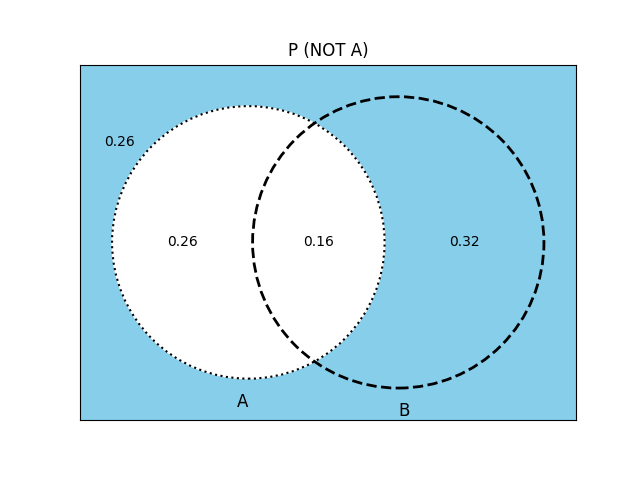
\includegraphics[scale=0.3]{Figure_1.png}
    \caption{P(not A)}
    \label{fig:1}
\end{figure}

\end{columns}
\end{frame}


\subsection{(ii) Determine p(not B)}
\begin{frame}{(ii) Determine p(not B)}
\begin{columns}

\column{0.5\textwidth}
Given $P(B) = 0.48$ so we have
${P(X=2) = 0.48}$
\begin{align*}
    P(B^\complement) &= 1 - P(X=2)\\ 
                    &= 1 - 0.48\\   
                    &= 0.52
\end{align*}
\begin{equation}
 \therefore P(not\ B) = 0.52   
\end{equation}

\column{0.5\textwidth}
\begin{figure}
    \centering
    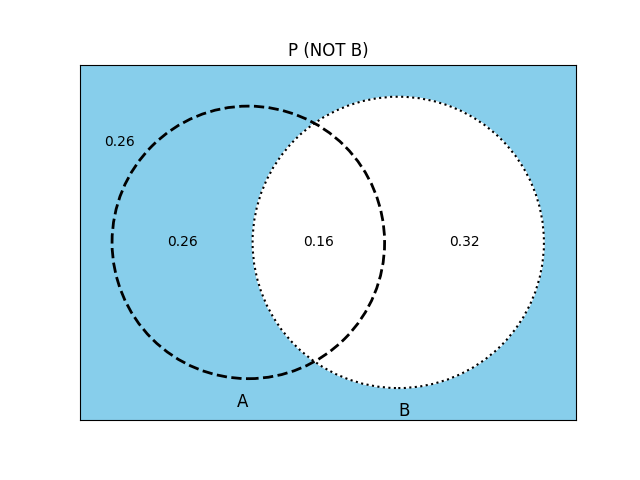
\includegraphics[scale=0.3]{Figure_2.png}
    \caption{P(not B)}
    \label{fig:2}
\end{figure}
\end{columns}
\end{frame}

\subsection{(iii) Determine p(A or B)}
\begin{frame}{(iii) Determine p(A or B)}\small
\begin{columns}
\column{0.5\textwidth}
Given ${P(A \cap\ B) = 0.16}$ , ${P(A) = 0.42}$ 
${P(B) =0.48}$ so we have\\
${\probinter =0.16}$
\begin{align*}
    \probunion &=P(X=1) + P(X=2)\\ 
               & - \probinter \\   
                &= 0.42 + 0.48 - 0.16 \\  
                &= 0.74 
\end{align*}
\column{0.5\textwidth}
\begin{center}
\begin{equation}
    \therefore P(A\ or \ B) = 0.74 
\end{equation}
\end{center}
\begin{figure}
    \centering
    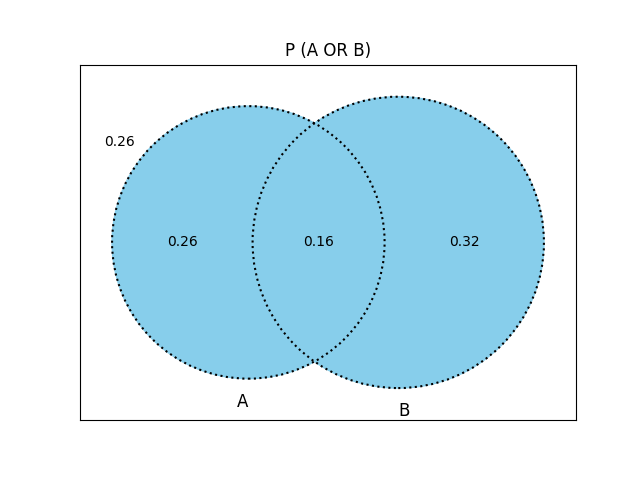
\includegraphics[scale=0.3]{Figure_3.png}
    \caption{$P(A \cup\ B)$}
    \label{fig:3}
\end{figure}
\end{columns}
\end{frame}

\section{verification}
\begin{frame}{Verification}
\begin{figure}
    \textbf{\textit{Verification}} \\
    \centering
    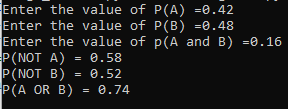
\includegraphics[scale=1]{Figure_4.png}
    \caption*{python code}
    \label{fig_code}
\end{figure}
\end{frame}

\end{document}